\chapter{Anexo referente às imagens dos gráficos utilizados no relatório (TripAdvisor - gráficos temporais)}
\label{an6}

Acesso aos ficheiros \textit{PowerBI} criados e as imagens retiradas do mesmo:

\begin{enumerate}
    \item \href{https://github.com/CatKinKitKat/pi2021/blob/master/projecto/sql/Graphs.pbix}{GitHub gráficos PowerBI 1}.
    \item \href{https://github.com/CatKinKitKat/pi2021/blob/master/projecto/sql/qq.pbix}{GitHub gráficos PowerBI 2}.
    \item \href{https://github.com/CatKinKitKat/pi2021/tree/master/projecto/sql/screenshotsPowerBI}{GitHub PowerBI screenshots}.
    \item \href{https://github.com/CatKinKitKat/pi2021/tree/master/projecto/datascience/sql/wordclouds}{GitHub wordclouds}
    \item \href{https://github.com/CatKinKitKat/pi2021/tree/master/projecto/datascience/sql/graphs/keywords}{GitHub gráficos Keywords}
    \item \href{https://github.com/CatKinKitKat/pi2021/tree/master/projecto/datascience/sql/graphs/sentiments}{GitHub gráficos Sentimentos}
\end{enumerate}

\begin{figure}[!htb]
\centering
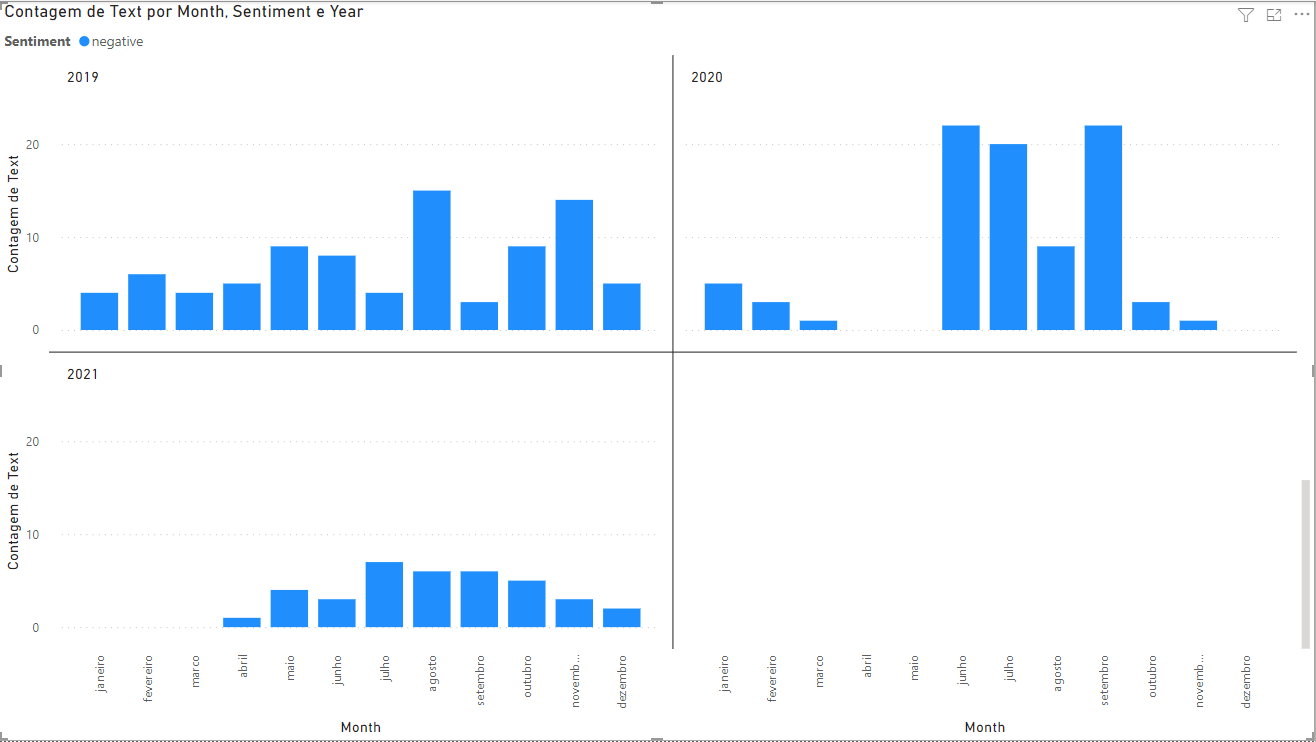
\includegraphics[width=7cm]{figuras/NegPerYear/4.PNG}
\caption{Gráfico de barras gerado baseando-se nos \textit{sentiments} mais usados da plataforma \textit{TripAdvisor} com níveis temporais sobre os \textit{sentiments} negativos ao longo do tempo}
\label{fig:exemplofig}
\end{figure}

\begin{figure}[!htb]
\centering
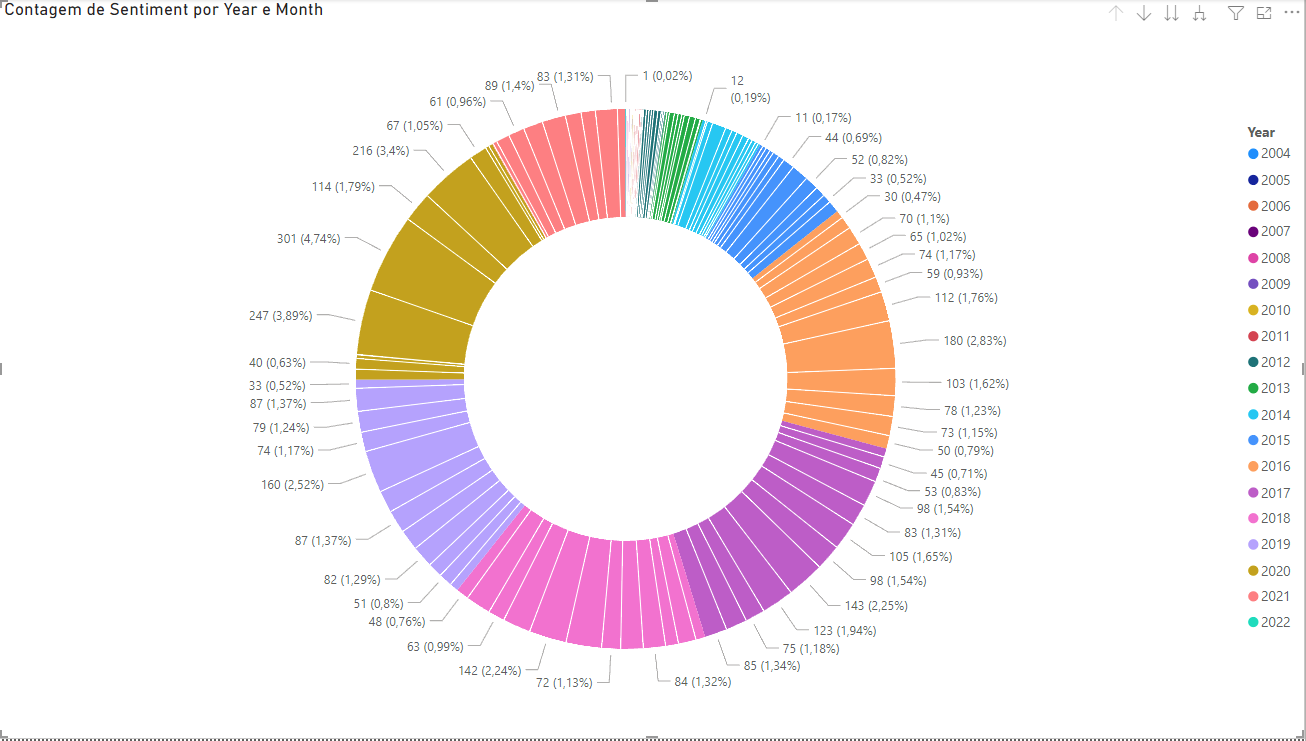
\includegraphics[width=7cm]{figuras/NrReviewsPerYear/CircleGraph.PNG}
\caption{Gráfico circular gerado baseando-se no número de \textit{sentiments} da plataforma \textit{TripAdvisor} ao longo dos anos}
\label{fig:exemplofig}
\end{figure}

\begin{figure}[!htb]
\centering
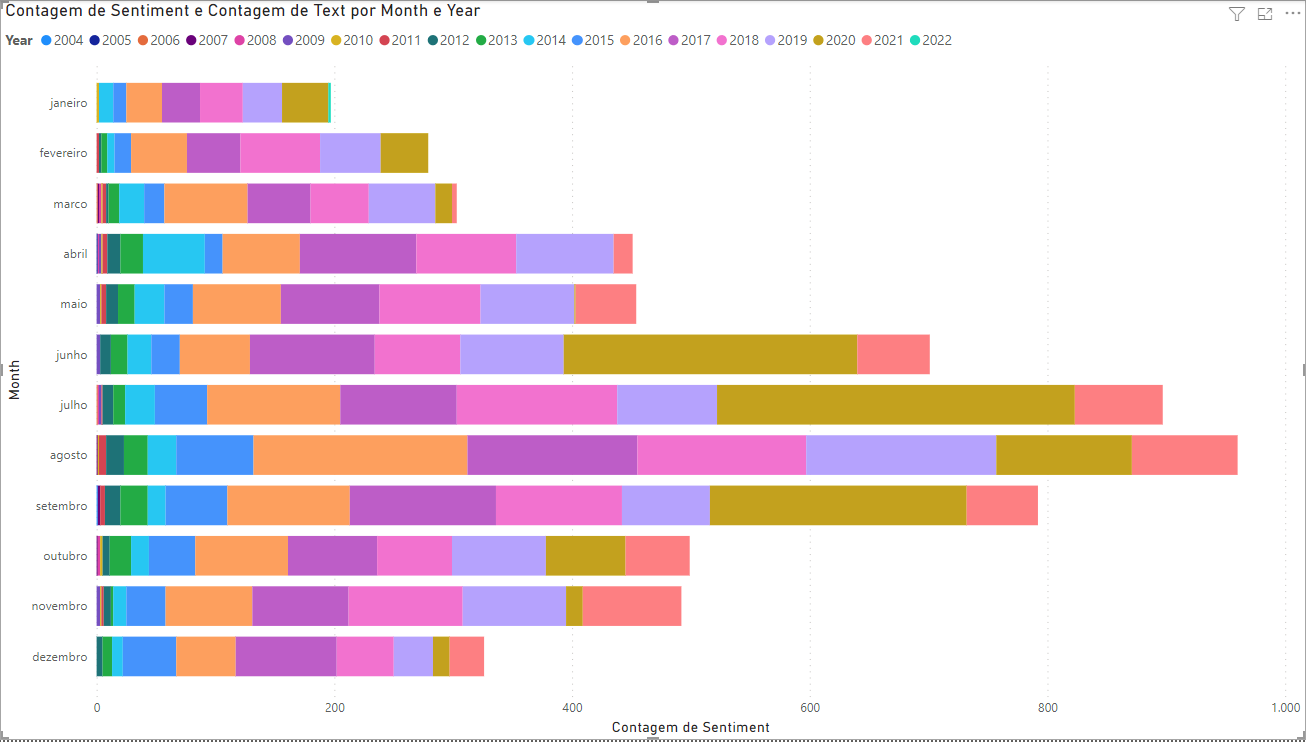
\includegraphics[width=7cm]{figuras/NrReviewsPerYear/TableGraph6.PNG}
\caption{Gráfico de barras gerado baseando-se no número de \textit{sentiments} da plataforma \textit{TripAdvisor} ao longo dos anos}
\label{fig:exemplofig}
\end{figure}

\begin{figure}[!htb]
\centering
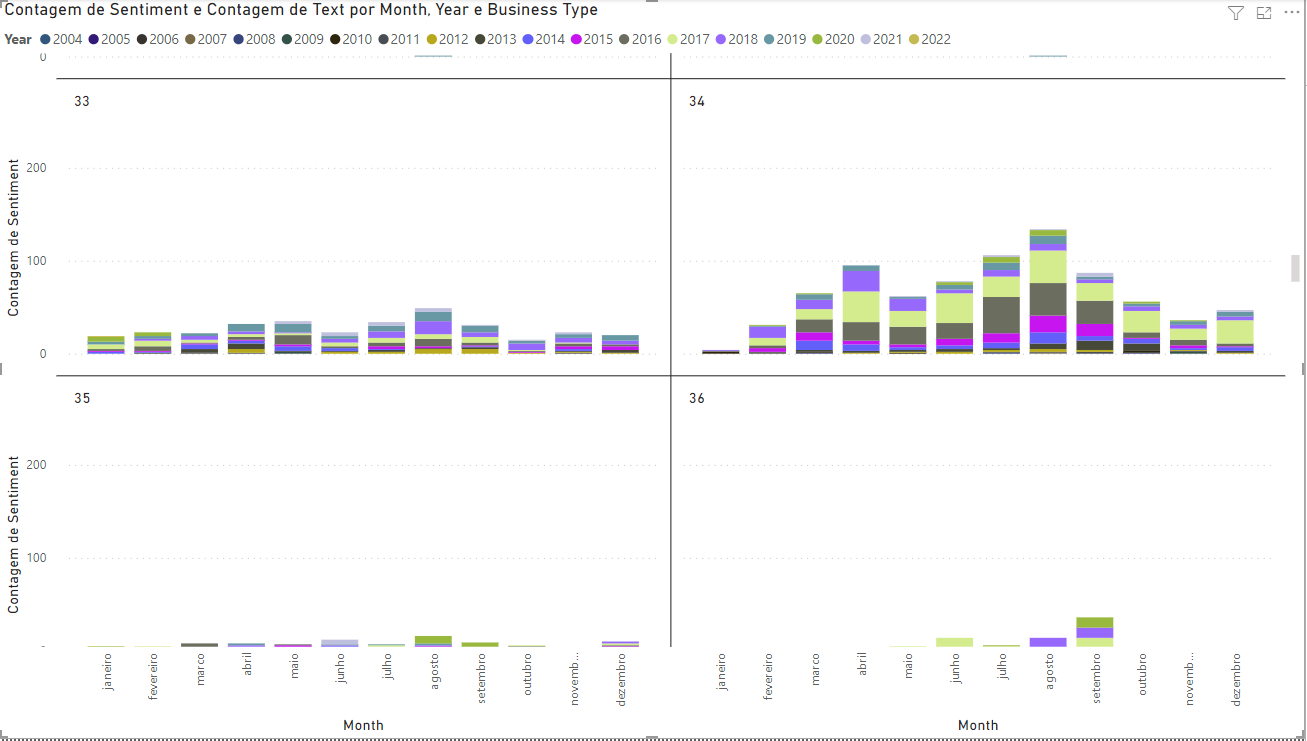
\includegraphics[width=7cm]{figuras/NrReviewsPerYear&BusinessType/5.PNG}
\caption{Gráfico de barras gerado baseando-se nos \textit{sentiments} mais usados e em cada hotel da plataforma \textit{TripAdvisor} ao longo dos anos}
\label{fig:exemplofig}
\end{figure}

\begin{figure}[!htb]
\centering
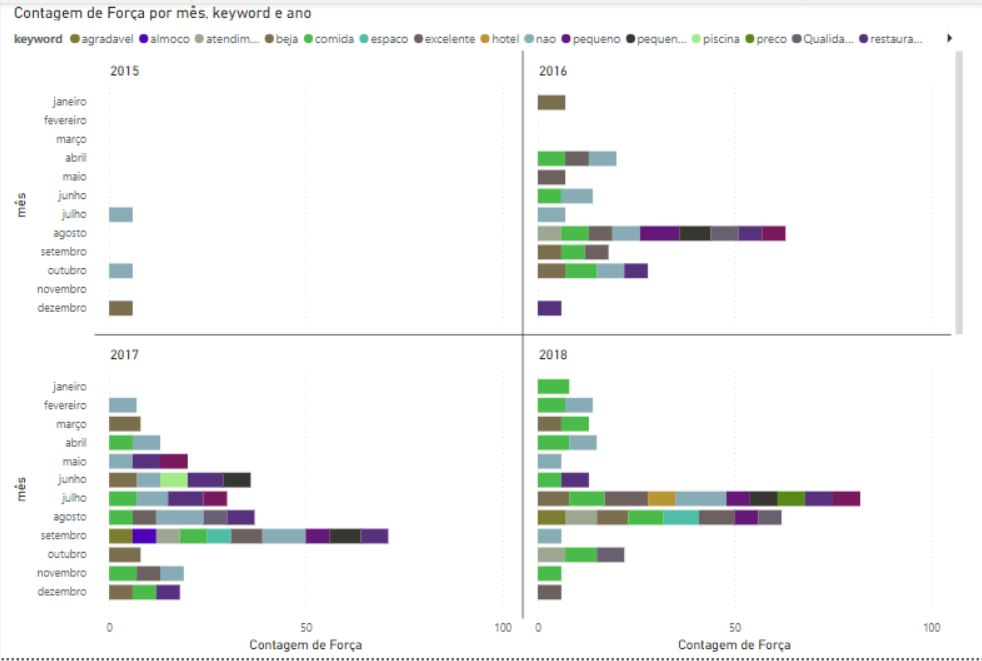
\includegraphics[width=7cm]{figuras/Keyword/keyword mais usadas para cada ano.JPG}
\caption{Gráfico de barras gerado baseando-se nas \textit{keywords} mais usadas dos hotéis da plataforma \textit{TripAdvisor} ao longo dos anos}
\label{fig:exemplofig}
\end{figure}

\begin{figure}[!htb]
\centering
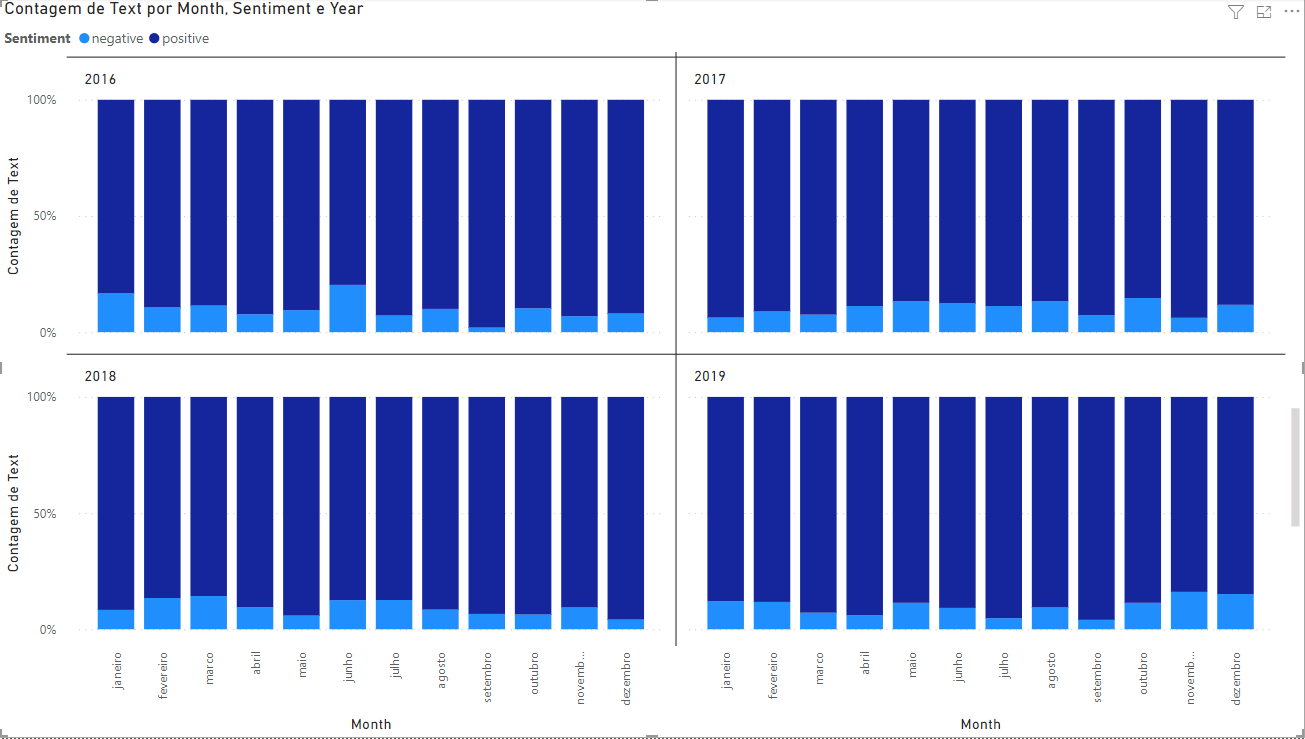
\includegraphics[width=7cm]{figuras/Pos&NegSentiments/TableGraph4.PNG}
\caption{Gráfico de barras gerado baseando-se nos \textit{sentiments} positivos e negativos dos hotéis da plataforma \textit{TripAdvisor} ao longo dos anos}
\label{fig:exemplofig}
\end{figure}

\begin{figure}[!htb]
\centering
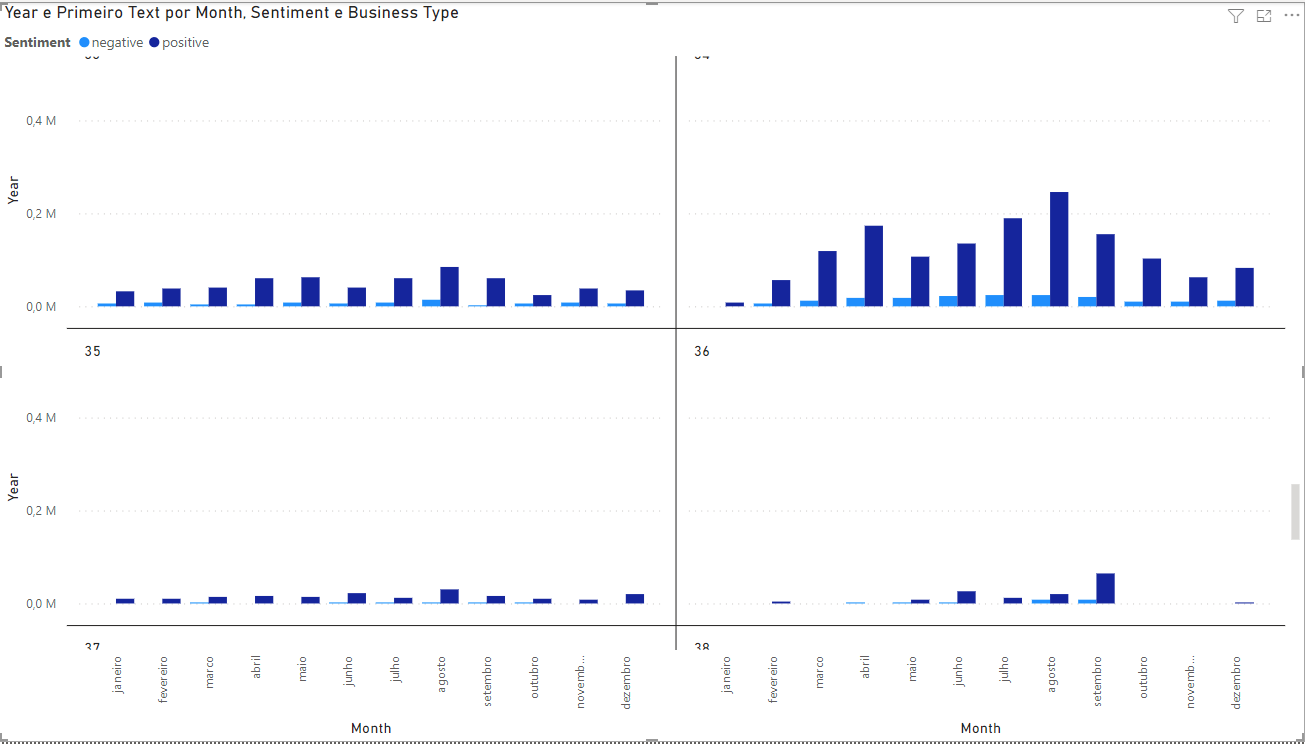
\includegraphics[width=7cm]{figuras/Pos&NegSentimentsPerMonth&BusinessType/2.PNG}
\caption{Gráfico de barras gerado baseando-se nos \textit{sentiments} positivos e negativos da plataforma \textit{TripAdvisor} ao longo dos anos em cada hotel}
\label{fig:exemplofig}
\end{figure}

\begin{figure}[!htb]
\centering
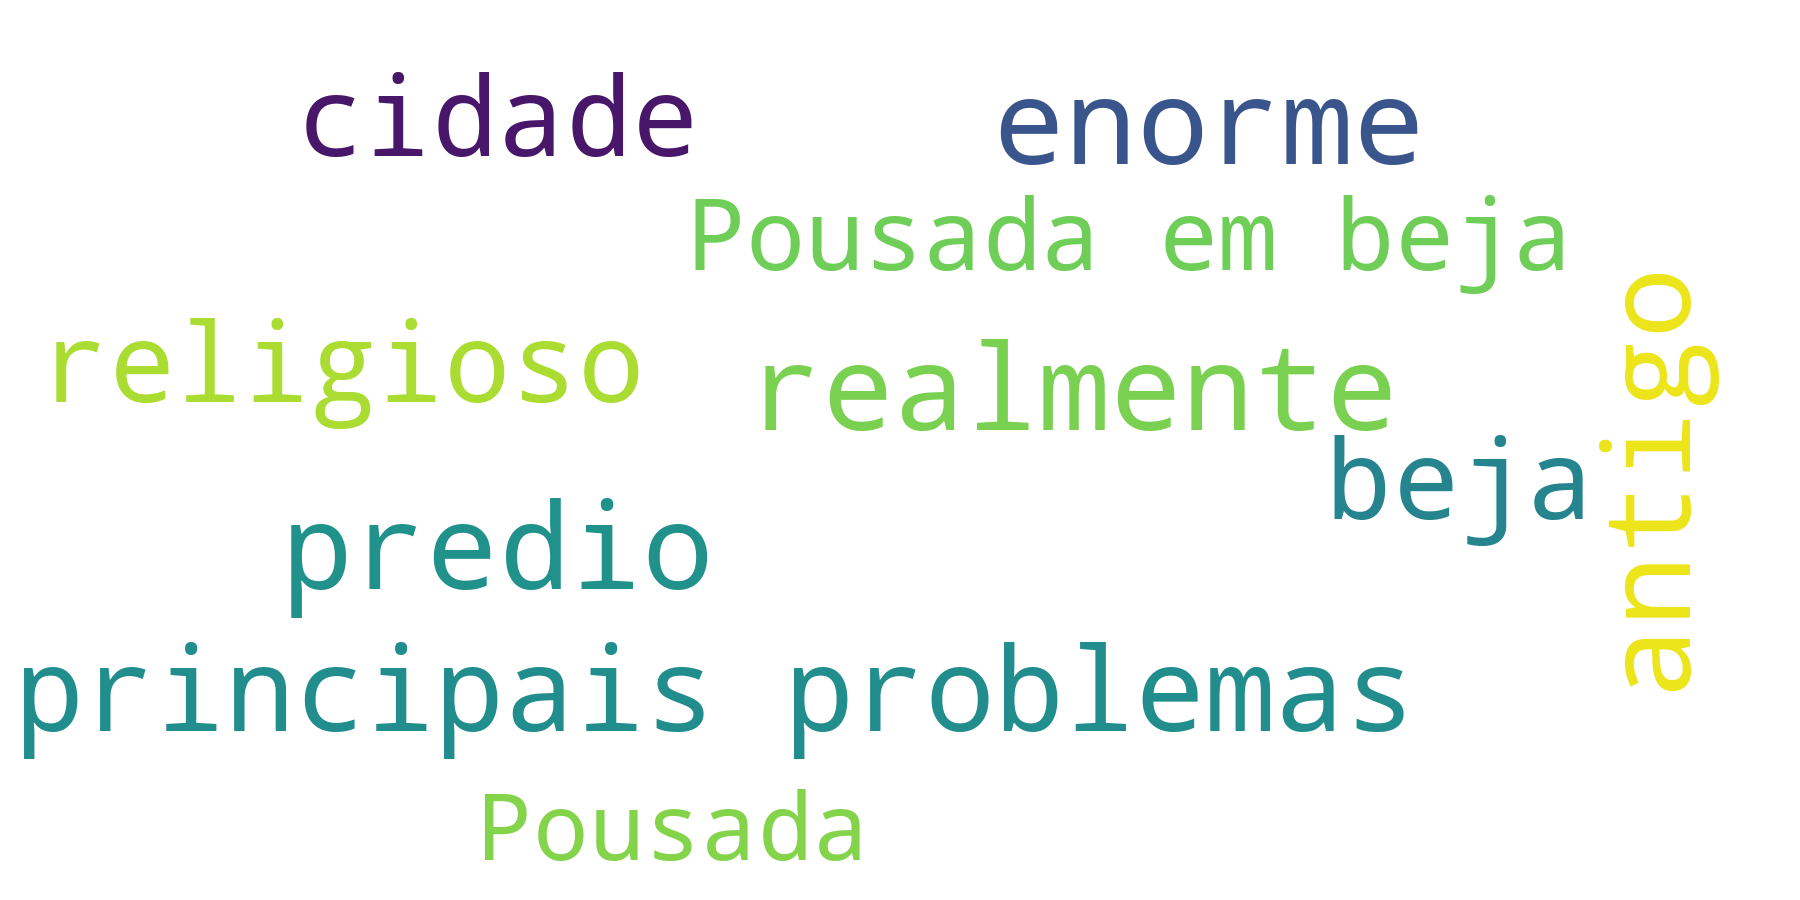
\includegraphics[width=7cm]{figuras/WordClouds/wordcloud_abril_of_2011_at_business33.png}
\caption{WordCloud gerado baseando-se nas \textit{keywords} mais usadas no Núcleo Museológico no Mês de Abril em 2011}
\label{fig:exemplofig}
\end{figure}

\begin{figure}[!htb]
\centering
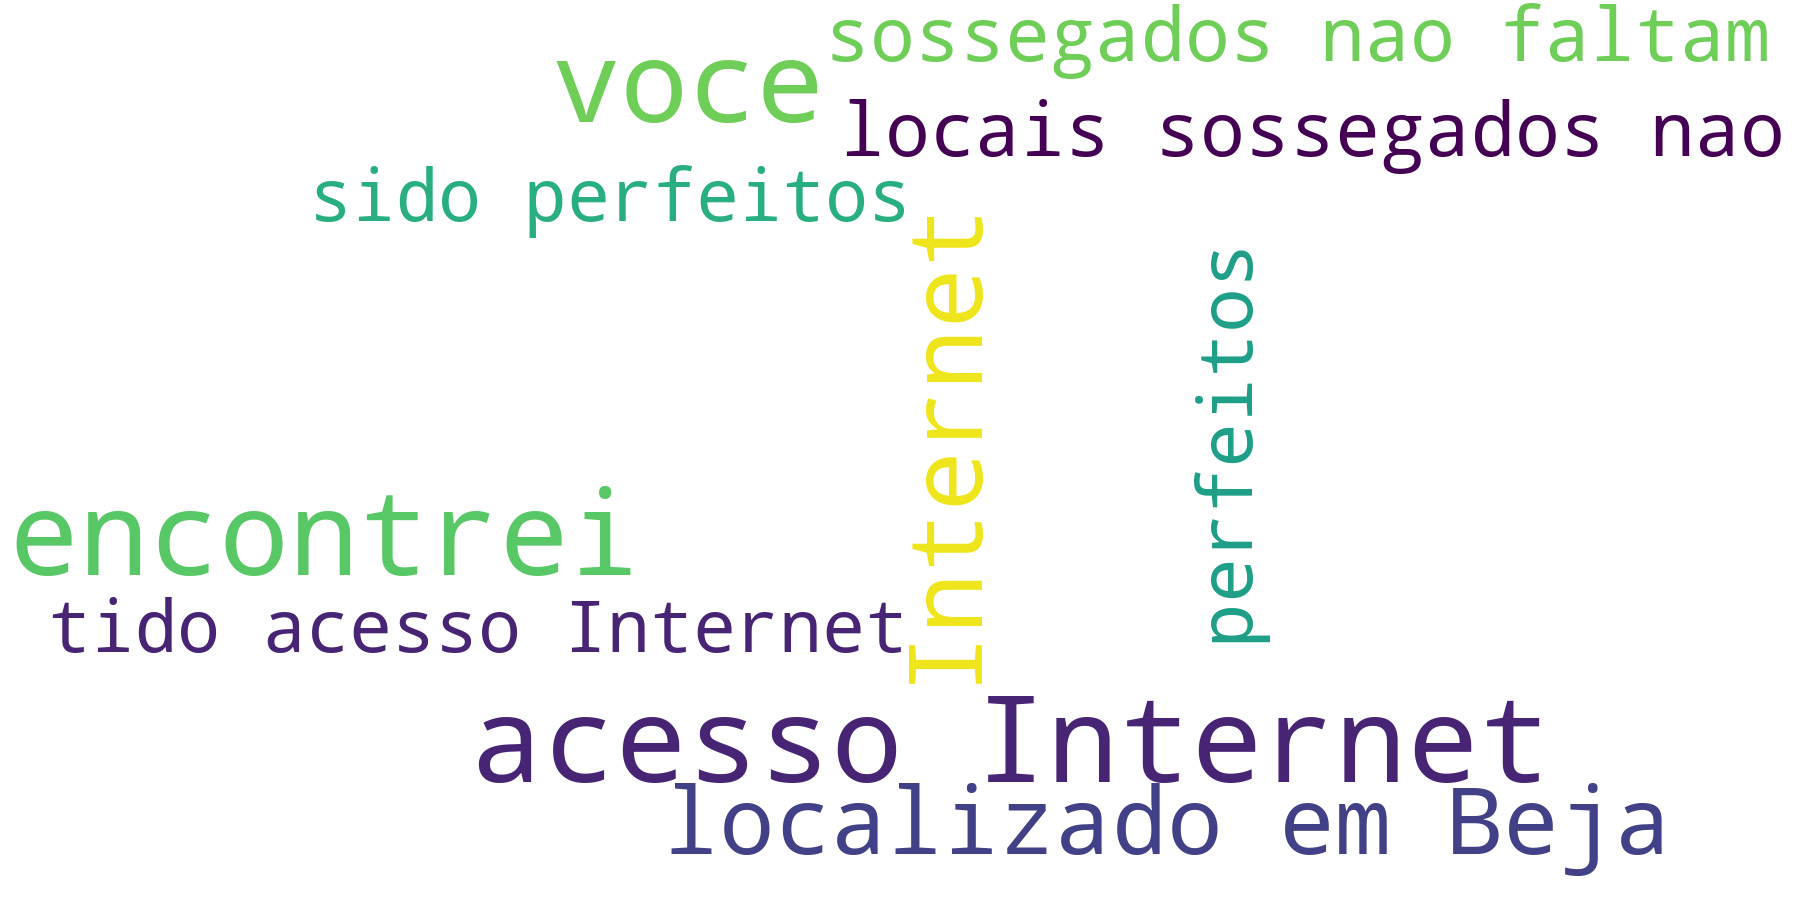
\includegraphics[width=7cm]{figuras/WordClouds/wordcloud_agosto_of_2012_at_business33.png}
\caption{WordCloud gerado baseando-se nas \textit{keywords} mais usadas no Núcleo Museológico no Mês de Agosto em 2012}
\label{fig:exemplofig}
\end{figure}

\begin{figure}[!htb]
\centering
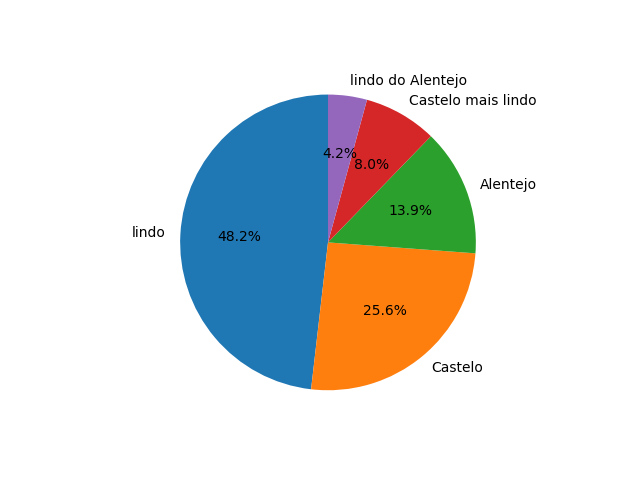
\includegraphics[width=7cm]{figuras/Graficos_Circulares_keyword/circular_keywords_agosto_of_2012_at_business2.png}
\caption{Gráfico circular com as percentagens das \textit{keywords} mais usadas do Restaurante Dom Dinis no Mês de Agosto em 2012}
\label{fig:exemplofig}
\end{figure}

\begin{figure}[!htb]
\centering
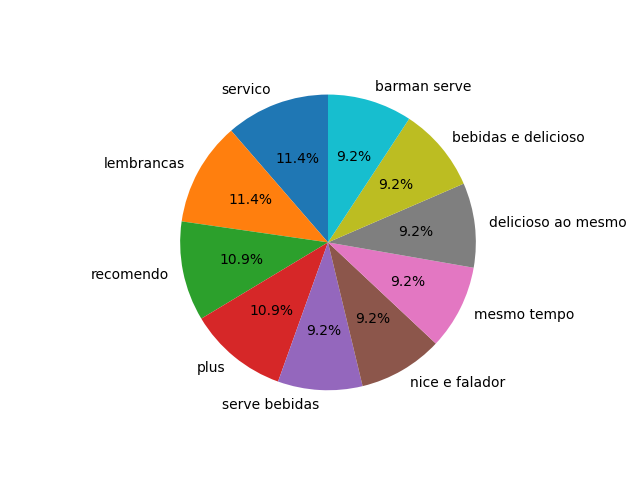
\includegraphics[width=7cm]{figuras/Graficos_Circulares_keyword/circular_keywords_abril_of_2013_at_business39.png}
\caption{Gráfico circular com as percentagens das \textit{keywords} mais usadas na Sé Catedral Beja no Mês de Abril em 2013}
\label{fig:exemplofig}
\end{figure}

\begin{figure}[!htb]
\centering
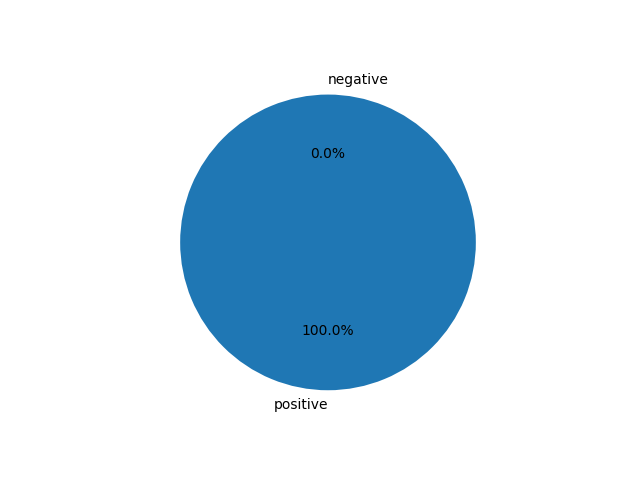
\includegraphics[width=7cm]{figuras/graficos_circulares_sent/circular_sentiment_abril_of_2011_at_business33.png}
\caption{Gráfico circular com a opinião positiva e negativa no Núcleo Museológico no Mês de Abril em 2011}
\label{fig:exemplofig}
\end{figure}

\begin{figure}[!htb]
\centering
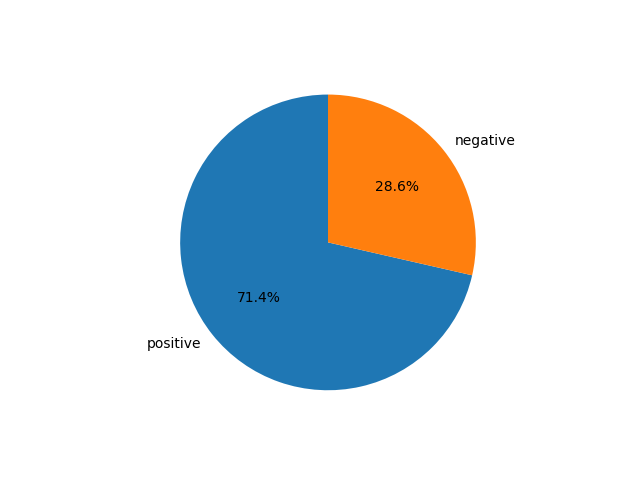
\includegraphics[width=7cm]{figuras/graficos_circulares_sent/circular_sentiment_abril_of_2014_at_business34.png}
\caption{Gráfico circular com a opinião positiva e negativa na Casa Santa Vitoria no Mês de Abril em 2014}
\label{fig:exemplofig}
\end{figure}